\documentclass[14pt,a4paper]{report}  %紙張設定
\usepackage{xeCJK}%中文字體模組
%\setCJKmainfont{標楷體} %設定中文字體
\setCJKmainfont{MoeStandardKai.ttf}
%\newfontfamily\sectionef{Times New Roman}%設定英文字體
\newfontfamily\sectionef{Nimbus Roman}
\usepackage{enumerate}
\usepackage{amsmath,amssymb}%數學公式、符號
\usepackage{amsfonts} %數學簍空的英文字
\usepackage{graphicx, subfigure}%圖形
\usepackage{fontawesome5} %引用icon
\usepackage{type1cm} %調整字體絕對大小
\usepackage{textpos} %設定文字絕對位置
\usepackage[top=2.5truecm,bottom=2.5truecm,
left=3truecm,right=2.5truecm]{geometry}
\usepackage{titlesec} %目錄標題設定模組
\usepackage{titletoc} %目錄內容設定模組
\usepackage{textcomp} %表格設定模組
\usepackage{multirow} %合併行
%\usepackage{multicol} %合併欄
\usepackage{CJK} %中文模組
\usepackage{CJKnumb} %中文數字模組
\usepackage{wallpaper} %浮水印
\usepackage{listings} %引用程式碼
\usepackage{hyperref} %引用url連結
\usepackage{setspace}
\usepackage{lscape}%設定橫式
\lstset{language=Python, %設定語言
		basicstyle=\fontsize{10pt}{2pt}\selectfont, %設定程式內文字體大小
		frame=lines,	%設定程式框架為線
}
%\usepackage{subcaption}%副圖標
\graphicspath{{./../images/}} %圖片預設讀取路徑
\usepackage{indentfirst} %設定開頭縮排模組
\renewcommand{\figurename}{\Large 圖.} %更改圖片標題名稱
\renewcommand{\tablename}{\Large 表.}
\renewcommand{\lstlistingname}{\Large 程式.} %設定程式標示名稱
\hoffset=-5mm %調整左右邊界
\voffset=-8mm %調整上下邊界
\setlength{\parindent}{3em}%設定首行行距縮排
\usepackage{appendix} %附錄
\usepackage{diagbox}%引用表格
\usepackage{multirow}%表格置中
%\usepackage{number line}
%=------------------更改標題內容----------------------=%
\titleformat{\chapter}[hang]{\center\sectionef\fontsize{20pt}{1pt}\bfseries}{\LARGE 第\CJKnumber{\thechapter}章}{1em}{}[]
\titleformat{\section}[hang]{\sectionef\fontsize{18pt}{2.5pt}\bfseries}{{\thesection}}{0.5em}{}[]
\titleformat{\subsection}[hang]{\sectionef\fontsize{18pt}{2.5pt}\bfseries}{{\thesubsection}}{1em}{}[]
%=------------------更改目錄內容-----------------------=%
\titlecontents{chapter}[11mm]{}{\sectionef\fontsize{18pt}{2.5pt}\bfseries\makebox[3.5em][l]
{第\CJKnumber{\thecontentslabel}章}}{}{\titlerule*[0.7pc]{.}\contentspage}
\titlecontents{section}[18mm]{}{\sectionef\LARGE\makebox[1.5em][l]
{\thecontentslabel}}{}{\titlerule*[0.7pc]{.}\contentspage}
\titlecontents{subsection}[4em]{}{\sectionef\Large\makebox[2.5em][l]{{\thecontentslabel}}}{}{\titlerule*[0.7pc]{.}\contentspage}
%=----------------------章節間距----------------------=%
\titlespacing*{\chapter} {0pt}{0pt}{18pt}
\titlespacing*{\section} {0pt}{12pt}{6pt}
\titlespacing*{\subsection} {0pt}{6pt}{6pt}
%=----------------------標題-------------------------=%             
\begin{document} %文件
\sectionef %設定英文字體啟用
\vspace{12em}
\begin{titlepage}%開頭
\begin{center}   %標題  
\makebox[1.5\width][s] %[s] 代表 Stretch the interword space in text across the entire width
{\fontsize{24pt}{2.5pt}國立虎尾科技大學}\\[18pt]
\makebox[1.5\width][s]
{\fontsize{24pt}{2.5pt}機械設計工程系}\\[18pt]
\sectionef\fontsize{24pt}{1em}\selectfont\textbf
{
\vspace{0.5em}
cd2023 2a3-pj3ag1分組報告}\\[18pt]
%設定文字盒子 [方框寬度的1.5倍寬][對其方式為文字平均分分布於方框中]\\距離下方18pt
\vspace{1em} %下移
\fontsize{30pt}{1pt}\selectfont\textbf{網際足球對戰場景設計}\\
\vspace{1em}
\sectionef\fontsize{30pt}{1em}\selectfont\textbf
{
\vspace{0.5em}
Web-based Foosball Scene Design}
 \vspace{2em}
%=---------------------參與人員-----------------------=%             
\end{center}
\begin{flushleft}
\begin{LARGE}

\hspace{32mm}\makebox[5cm][s]
{指導教授:\quad 嚴\quad 家\quad 銘\quad 老\quad 師}\\[6pt]
\hspace{32mm}\makebox[5cm][s]
{班\qquad 級:\quad 四\quad 設\quad 二\quad 甲}\\[6pt]
\hspace{32mm}\makebox[5cm][s]
{學\qquad 生:\quad 王\quad 樟 \quad 皓\quad(41023114)}
\\[6pt]
\hspace{32mm}\makebox[5cm][s]
{\hspace{36.5mm}吳\quad 政 \quad 憲\quad(41023118)}\\[6pt]
\hspace{32mm}\makebox[5cm][s]
{\hspace{36.5mm}呂\quad 承 \quad 劼\quad(41023119)組長}\\[6pt]
\hspace{32mm}\makebox[5cm][s]
{\hspace{36.5mm}呂\quad 昕 \quad 叡\quad(41023120)}\\[6pt]
\hspace{32mm}\makebox[5cm][s]
{\hspace{36.5mm}李\quad 彥 \quad 廷\quad(41023122)}\\[6pt]
\hspace{32mm}\makebox[5cm][s]
{\hspace{36.5mm}李\quad 茂 \quad 廷\quad(41023124)}\\[6pt]
\hspace{32mm}\makebox[5cm][s]
{\hspace{36.5mm}卓\quad 桓 \quad 琮\quad(41023126)}\\[6pt]
\hspace{32mm}\makebox[5cm][s]
{\hspace{36.5mm}林\quad 敬 \quad 燐\quad(41023138)}\\[6pt]
\end{LARGE}
\end{flushleft}
\vspace{6em}
\fontsize{18pt}{2pt}\selectfont\centerline{\makebox[\width][s]
{中華民國\hspace{3em} 
112 \quad 年\quad 6\quad 月}}
\end{titlepage}
\newpage
%=------------------------摘要-----------------------=%
\renewcommand{\baselinestretch}{1.5} %設定行距
\pagenumbering{roman} %設定頁數為羅馬數字
\clearpage  %設定頁數開始編譯
\sectionef
\addcontentsline{toc}{chapter}{摘~~~要} %將摘要加入目錄
\begin{center}
\LARGE\textbf{摘~~要}\\
\end{center}
\begin{flushleft}
\fontsize{14pt}{20pt}\sectionef\hspace{12pt}\quad 本課程將採兩人一組、四人一組與八人一組的方式進行協同機電整合產品開發,開發一款能在 web-based CoppeliaSim 場景中雙方或多方 (human or computer) 對玩的遊戲 (game) 產品。最後在 w16 現場發表八人協同四週後所完成的產品,在 w17 各組採 OBS + Teams 以影片發表所完成的協同產品。\\[12pt]

\end{flushleft}
\begin{center}
\fontsize{14pt}{20pt}\sectionef\hspace{12pt}\quad 課程一開始讓學員可以從 https://mde.tw/cd2023/content/BubbleRob.html 導引練習中,了解 CoppeliaSim 套件中的諸多功能以及用法,其中包括利用近接感測器偵測障礙物,並透過 Lua script 控制 bubbleRob 雙輪車的移動。為了讓各組學員了解在多人協同模式下,開發機電資產品流程中必須面臨的許多議題(若要直接在瀏覽器中建立多方協同的場景,可以透過 remote API(導引) 與 Visualization Stream 功能)。再接續專案一的雙輪車,改用 Python zmqRemoteAPI 進行控制,各分組需完成能在 Visualization Stream 瀏覽器中,跨網路雙方各控制一台雙輪車在足球場中進行對陣,且需設計一組能在雙方瀏覽器中進行計分的系統。最後各組需對雙輪車進行設計改良,以提升行進與對戰效能,各組需採 CAD 進行場景與多輪車零組件設計後,轉入足球場景中以鍵盤 arrow keys 與 wzas 等按鍵進行控制,對陣雙方每組將有四名輪車球員,且每兩人在同一台電腦上操作,完成後各組需在分組網站中提供所有相關檔案下載連結,且提供線上分組簡報與分組 pdf 報告連結。\\[12pt]

\end{flushleft}
\begin{center}
\fontsize{14pt}{20pt}\sectionef\hspace{12pt}\quad 專案場景必須要有感測器及記分板,讓進球後可以顯示分數在場景上,而記分板除了採用 LED 顯示計分外,也要以建立以機械轉盤傳動計分系統。另外建立計時器讓學員在對戰時得知時間剩多少,並利用程式控制球門使球重置後繼續對戰,最後在
CoppeliaSim 模擬環境中透過埠號及 http://[2001:288:6004:17:2023:cda:x:x]:23020/ 進行對戰及觀看。\\[12pt]
\newpage
%=--------------------Abstract----------------------=%
\renewcommand{\baselinestretch}{1.5} %設定行距
\addcontentsline{toc}{chapter}{Abstract} %將摘要加入目錄
\begin{center}
\LARGE\textbf\sectionef{Abstract}\\
\begin{flushleft}
\fontsize{14pt}{16pt}\sectionef\hspace{12pt}\quad This course will involve collaborative development of mechatronic integrated products in teams of two, four, and eight members. The objective is to create a web-based game product using CoppeliaSim, where two or more participants (humans or computers) can engage in gameplay within the virtual environment. At the end of the course, during week 16, the eight-member teams will present their completed products in a live demonstration. In week 17, each group will use OBS + Teams to present a video showcasing their collaborative product.\\[12pt]

\end{flushleft}
\begin{center}
\fontsize{14pt}{16pt}\sectionef\hspace{12pt}\quad At the beginning of the course, participants will be guided to practice and explore various functionalities and usage of the CoppeliaSim package through the link https://mde.tw/cd2023/content/BubbleRob.html. This includes using proximity sensors to detect obstacles and controlling the movement of the BubbleRob differential-drive robot using Lua script. In order to familiarize the teams with the challenges encountered in the development of mechatronic products in a multi-user collaborative mode, they will utilize the remote API (guided) and Visualization Stream feature to create a collaborative scenario directly in the web browser. Continuing from Project 1, the teams will switch to using Python zmqRemoteAPI for control. Each group will be required to establish a scenario where two BubbleRob robots, controlled by two separate users over the network, engage in a soccer match within the visualization stream browser. Additionally, the teams need to design a scoring system that can be accessed and displayed in the browsers of both users. In the final stage, each group will improve the design of their BubbleRob robot to enhance its movement and performance during the match. The groups will employ CAD software to design the scene and components of the robots. The control will be switched to using arrow keys and "wzas" keys on the keyboard to maneuver the robots within the soccer field. Each group will have four robot players, with each pair of participants operating on the same computer. Once completed, the groups are required to provide download links for all relevant files on the group website, along with links to online group presentations and PDF reports.\\[12pt]

\end{flushleft}
\begin{center}
\fontsize{14pt}{16pt}\sectionef\hspace{12pt}\quad 
The project scenario requires the presence of sensors and a scoreboard in the simulation environment. The scoreboard should display the score on the scene, indicating goals scored. Apart from using LED displays to show the score, a mechanical rotary-driven scoring system should also be implemented. Additionally, a timer needs to be created to inform the participants about the remaining time during the gameplay. The program should control the goal posts to reset the ball and continue the game. Finally, the participants can engage in the match and observe it through the CoppeliaSim simulation environment using the port address http://[2001:288:6004:17:2023:cda:x:x]:23020/. (Note: Please replace "x" in the provided address with the appropriate values or specific information.)\\[12pt]
\newpage
%=------------------------目錄----------------------=%
\renewcommand{\contentsname}{\centerline{\fontsize{18pt}{\baselineskip}\selectfont\textbf{目\quad 錄}}}
\tableofcontents  %目錄產生
\newpage
%=------------------圖表目錄產生----------------------=%
\renewcommand{\listfigurename}{\centerline{\fontsize{18pt}{\baselineskip}\selectfont\textbf{圖\quad 目\quad 錄 }}}
\newcommand{\loflabel}{圖} %定義\loflabel 文字為圖
\renewcommand{\numberline}[1]{\loflabel~#1\hspace*{0.5em}}
\listoffigures
%\newcommand{\captioname}{圖}
\end{center}

%=-------------------------內容----------------------=%
\chapter{前言}
\renewcommand{\baselinestretch}{10.0} %設定行距
\pagenumbering{arabic} %設定頁號阿拉伯數字
\setcounter{page}{1}  %設定頁數
\fontsize{14pt}{2.5pt}\sectionef
\section{專案概述與目標}
本課程專案目標需要有場景與多輪車零組件設計、控制程式、開會紀錄與逐字稿、各組員任務分配與執行過程影片及分組報告 pdf 檔案,最後在 w16 現場發表八人協同四週後所完成的產品,在 w17 各組採 OBS + Teams 以影片發表所完成的協同產品。
\begin{figure}[hbt!]
\begin{center}
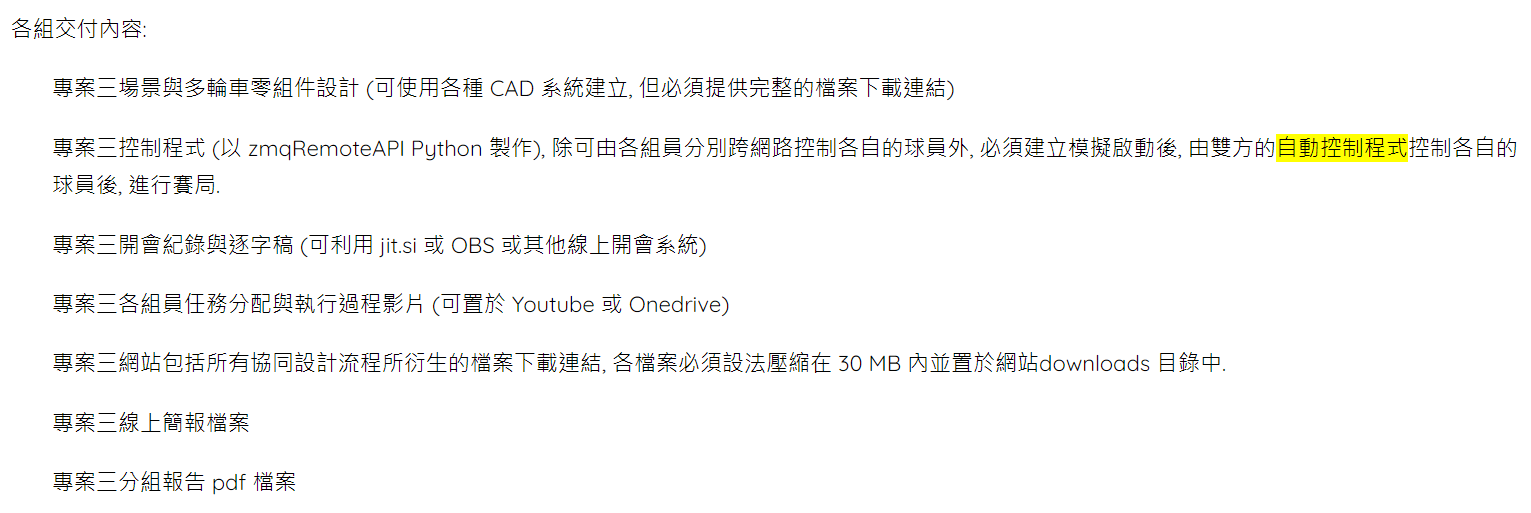
\includegraphics[height=5cm]{work}
\caption{\Large 專案目標}\label{專案目標}
\end{center}
\end{figure} 
\section{規則}
本專題設計理想為一款足球遊戲,比賽一開始球會置於場中央,遊戲開始後雙方即
可鍵盤操控機器人,透過隊友間的傳球並將球送至球門即可得分。\\
遊戲規則如下:\\
球送至敵方球門即得一分。\\
時間內進球數多的一方獲勝。\\
球進入球框後會回到原位。\\
球出界後會回到原位。\\
\renewcommand{\baselinestretch}{0.5} %設定行距
\chapter{專題設計}
\renewcommand{\baselinestretch}{10.0} %設定行距
\pagenumbering{arabic} %設定頁號阿拉伯數字
\setcounter{page}{2}  %設定頁數
\fontsize{14pt}{2.5pt}\sectionef

\section{尺寸規定}
在 https://mde.tw/cd2023/content/pj3.html 中規定球場及球員的大小及重量。\\
1. 足球規格:球為白色、直徑 0.1m、重量 0.5kg\\
2. 足球場地:長 4m x 寬 2.5m\\
3. 球門規格:長 0.6m, 高 0.3m, 寬 0.1m\\
4. 球員尺寸範圍:長寬高各 0.2m, 重量 5kg。\\

\section{建立球員}
本組使用 CoppeliaSim 內的 primitive shape 來製作車子,之所以使用簡單的形狀來製作車子是因為在模擬時車子細節太複雜會導致模擬運行速度變慢。由於初始的機器人為球型會導致在碰撞時容易翻倒,所以經過本組討論後在後續車體改良中更改為長方體使球員不容易翻倒。\\
\begin{figure}[hbt!]
\begin{center}
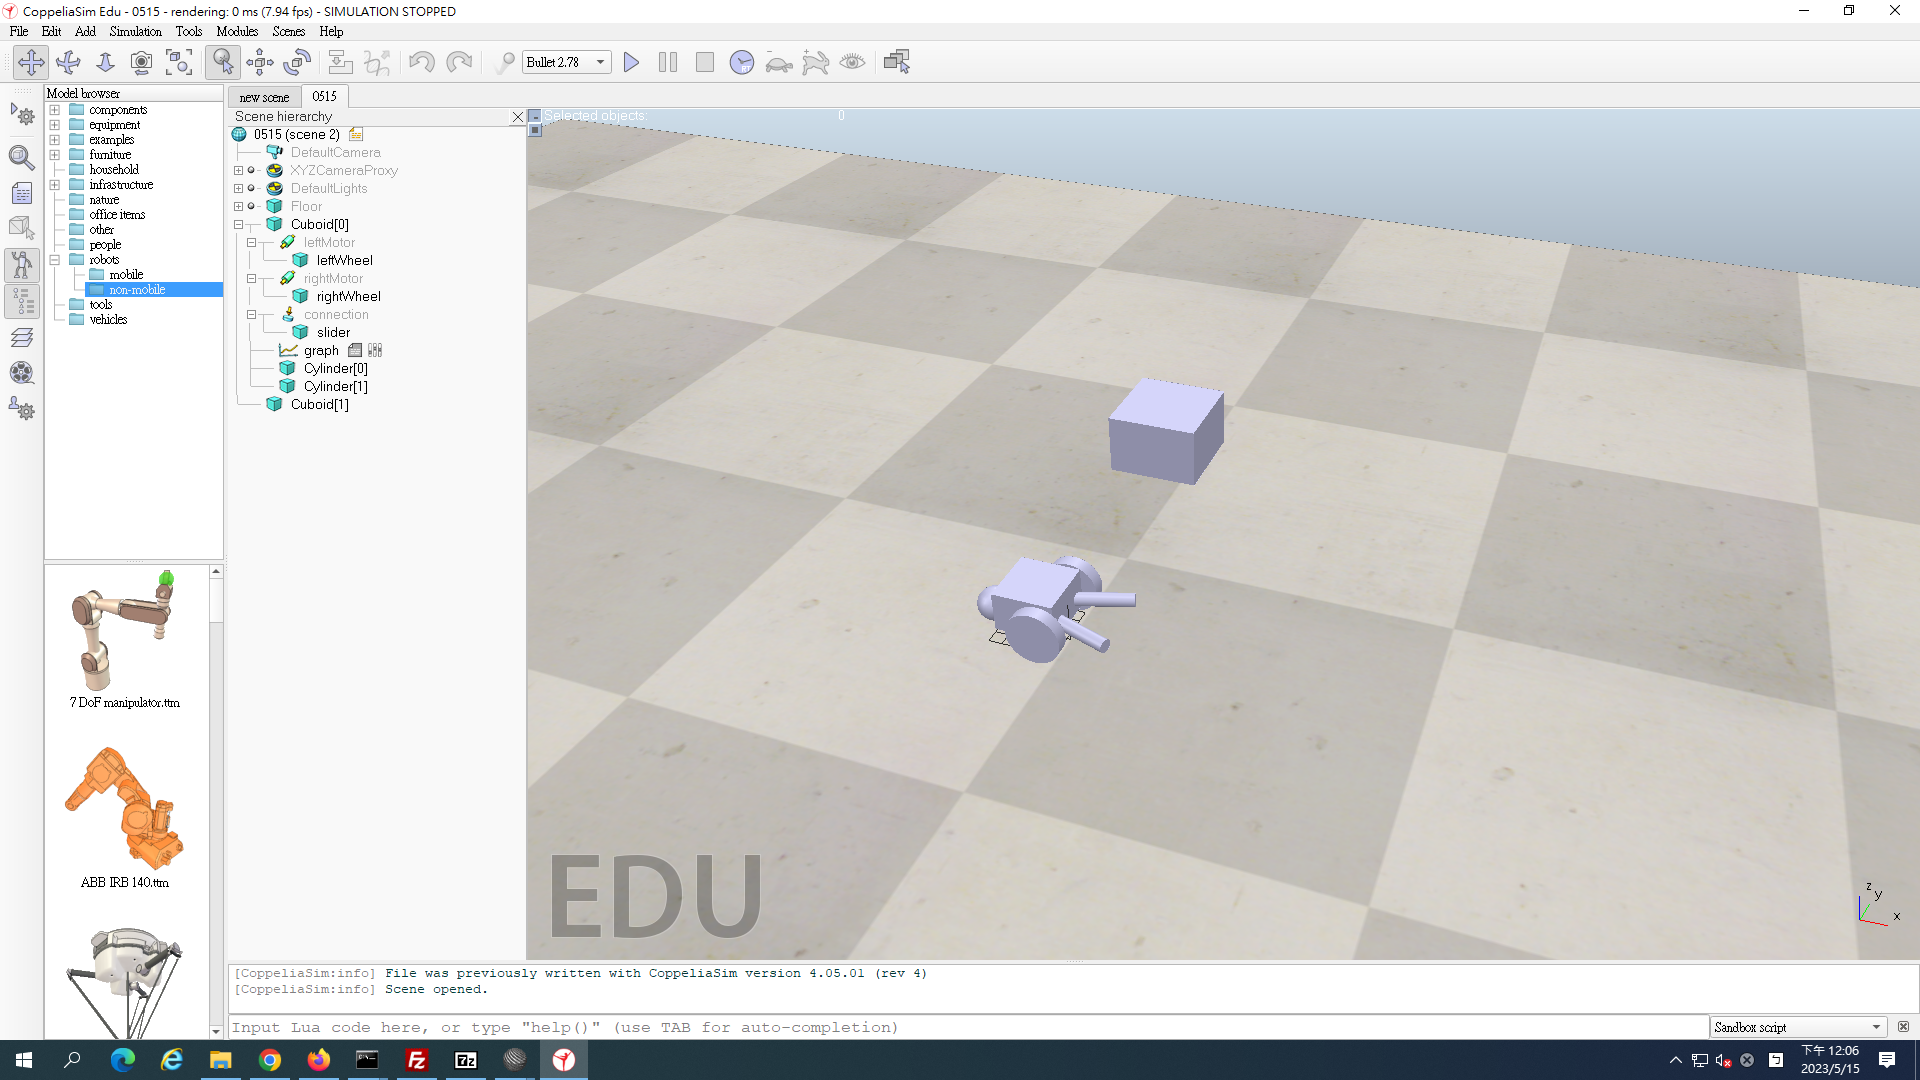
\includegraphics[width=10cm]{0515}
\caption{\Large 第一版車體}\label{車體}
\end{center}
\end{figure}

在執行控制車子程式時在移動左右轉彎時馬達產生偏移,後來發現是馬達座標設定錯誤直接而修改了定位,並且加上顏色及背號。\\
\begin{figure}[hbt!]
\begin{center}
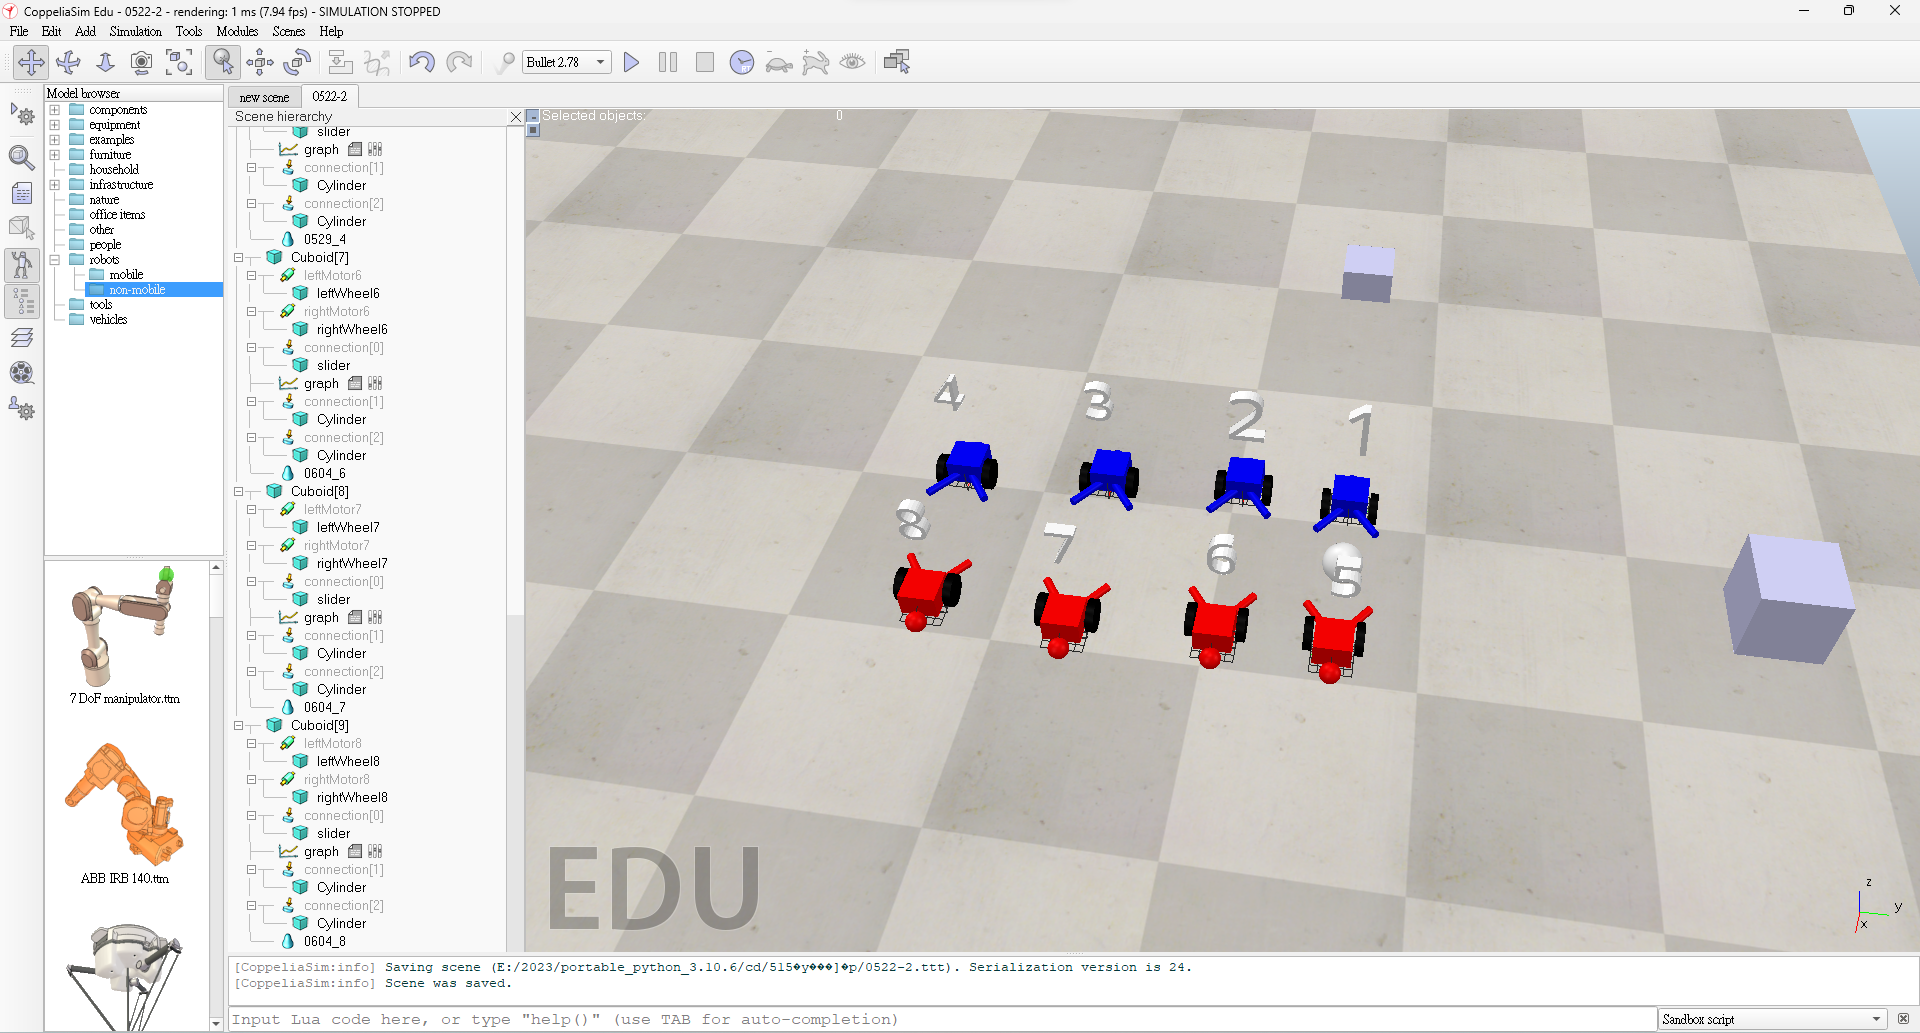
\includegraphics[width=12cm]{0604-1}
\caption{\Large 車體導入場景}\label{車體導入場景}
\end{center}
\end{figure}

\section{建立記分板}
本課程規定除了採用 LED 顯示計分外, 也要建立機械轉盤傳動計分系統。\\
LED 顯示計分是採用 NX 繪製出 stl 檔再導入 CoppeliaSim 中而程式部分後續會說明。\\
\begin{figure}[hbt!]
\begin{center}
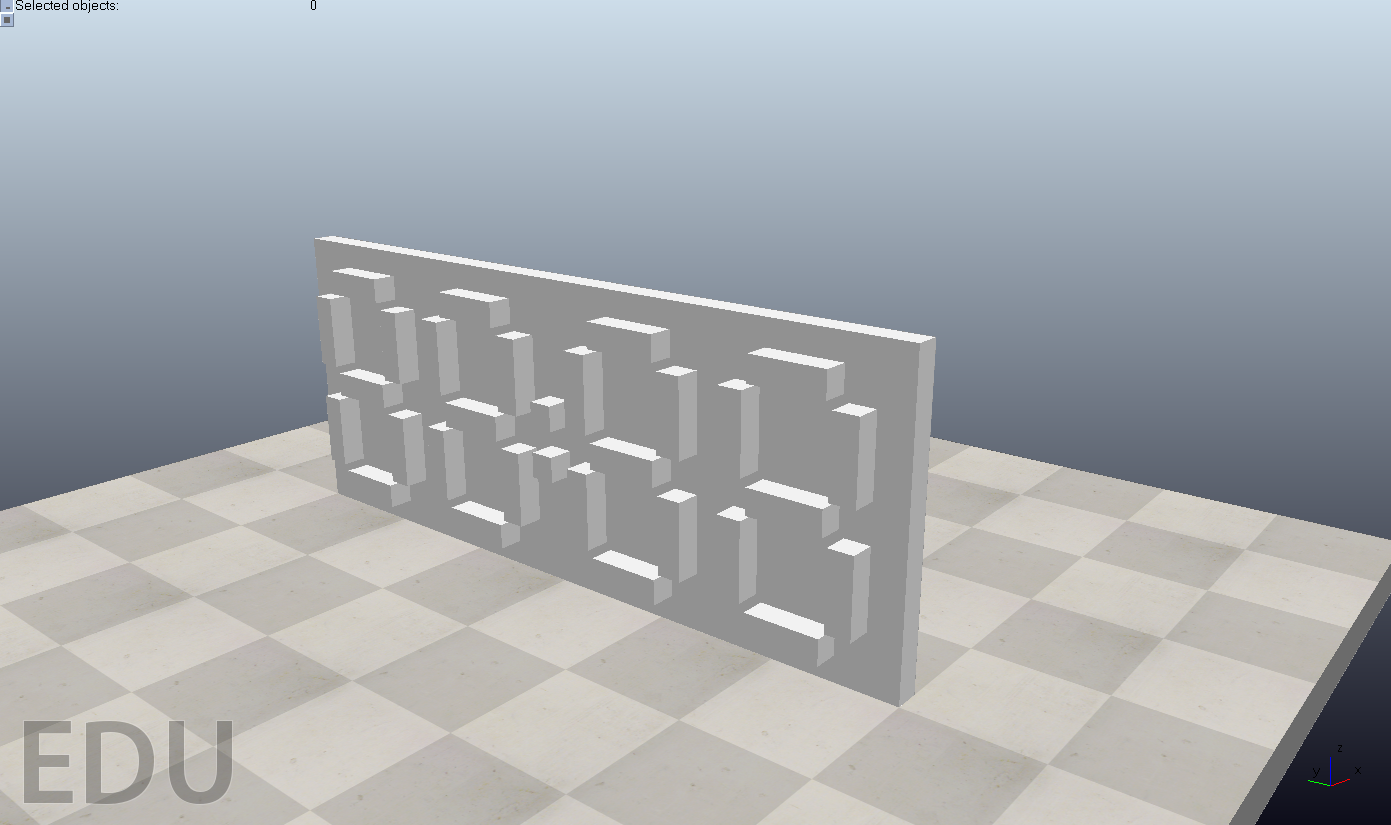
\includegraphics[width=10cm]{ledscore}
\caption{\Large 記分板建立}\label{記分板建立}
\end{center}
\end{figure}

機械轉盤傳動計分版是利用 onshape 繪製而成,並更改了顏色,但後續程式無法編譯出來而參考 pj3ag4 的機械式記分板。\\
\begin{figure}[hbt!]
\begin{center}
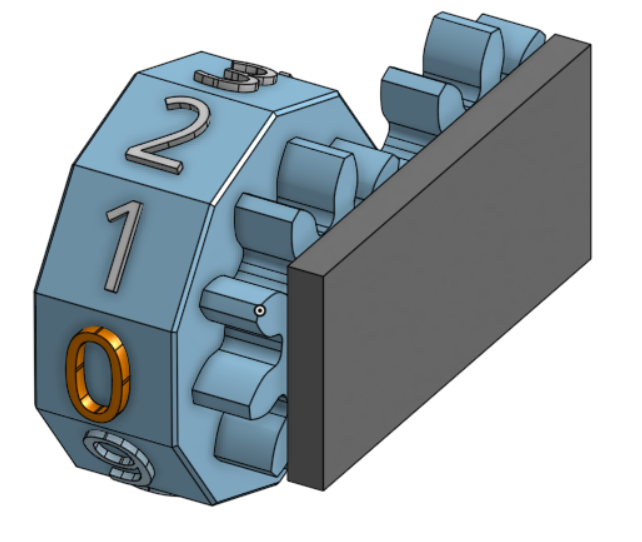
\includegraphics[width=8cm]{輪盤記分板-4-10teeth}
\caption{\Large 初版記分板}\label{初版記分板}
初版記分板 概念是由馬達帶動齒輪10齒輪傳動
\end{center}
\end{figure}
\begin{figure}[hbt!]
\begin{center}
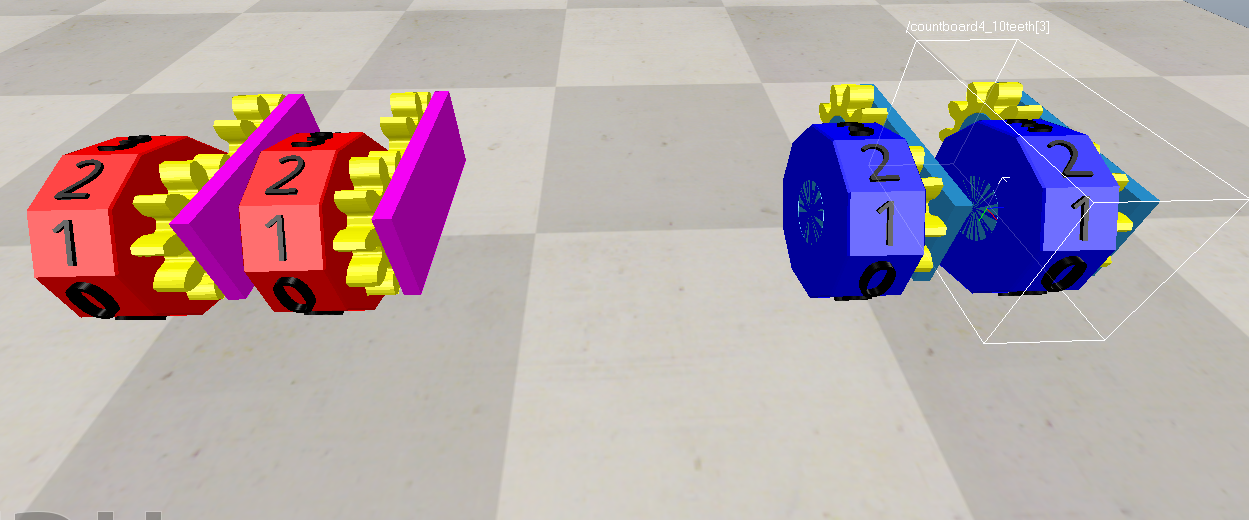
\includegraphics[width=8cm]{Screenshot 2023-05-29 113148.png4-10}
\caption{\Large 匯入記分板}\label{匯入記分板}
\end{center}
\end{figure}
\begin{figure}[hbt!]
\begin{center}
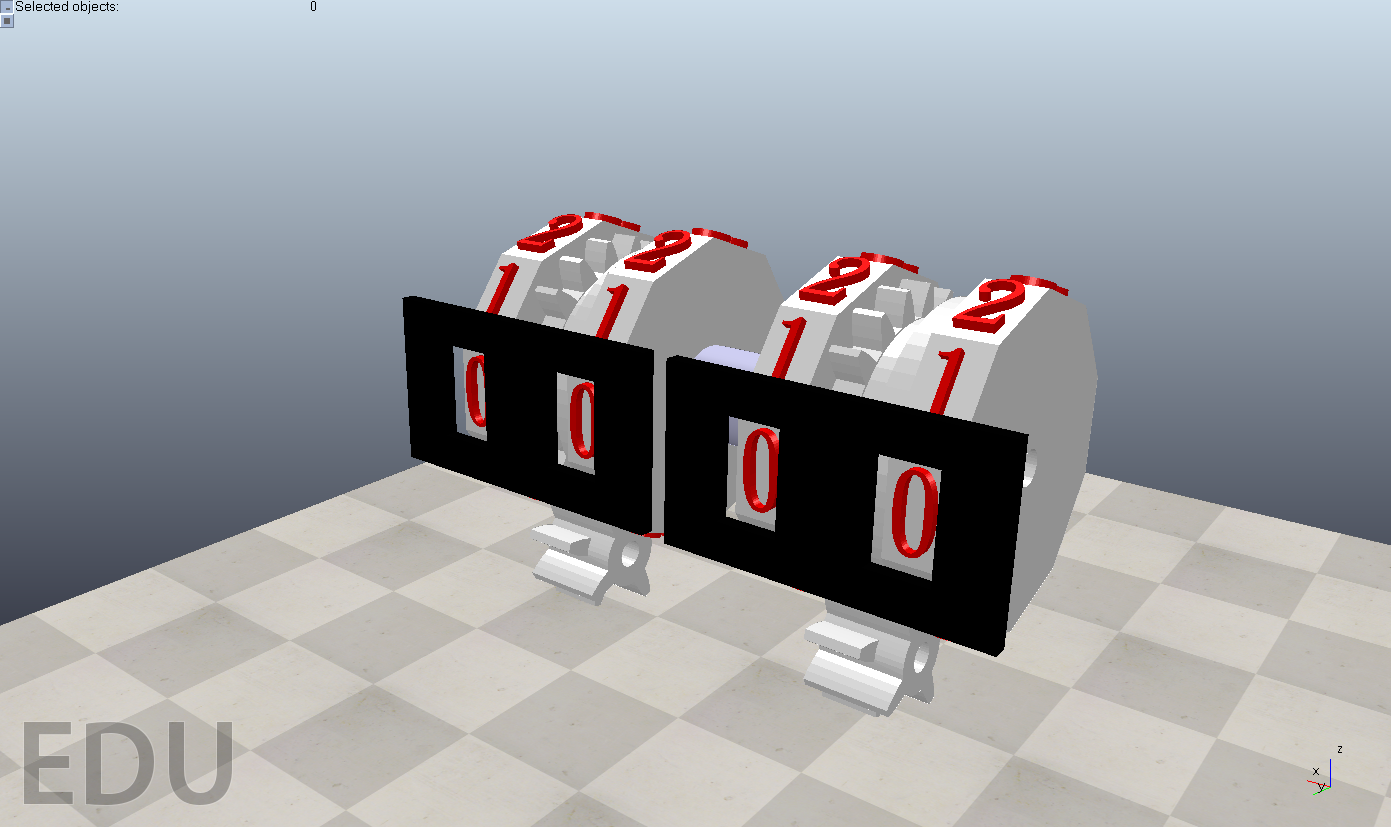
\includegraphics[width=8cm]{scoreboard}
\caption{\Large 匯入第二版記分板}\label{匯入最終版記分板}
最終版記分板 是由齒輪組傳動 20齒及10齒和二階傳動輪組成
\end{center}
\end{figure}
\begin{figure}
\begin{center}
詳細的記分板組成及製作過程 可以參考本組網頁:
\herf{https://mdecd2023.github.io/2a3-pj3ag1/content/%E8%BC%AA%E7%9B%A4%E8%A8%98%E5%88%86%E6%9D%BF%E7%B9%AA%E8%A3%BD.html}
\end{center}
\end{figure}

\section{建立計時器}
在進行比賽時需要有計時器讓參賽者得知比賽還多久結束,而計時器模型則是沿用記分板之檔案。\\
\begin{figure}[hbt!]
\begin{center}
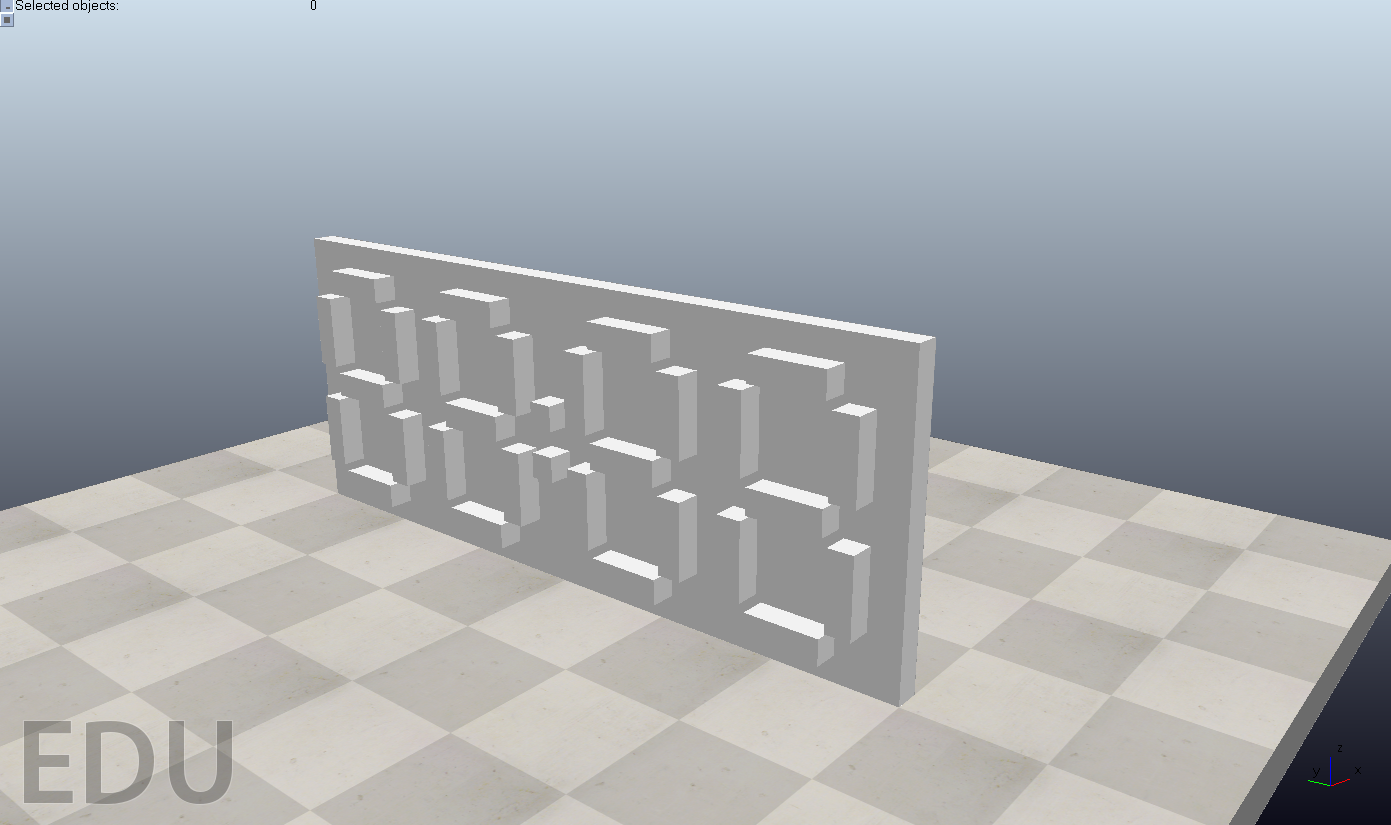
\includegraphics[width=8cm]{ledscore}
\caption{\Large 匯入記時器}\label{匯入記時器}
\end{center}
\end{figure}

\section{建立球場}
我們使用 Onshape 繪製了球場底板及球門,匯入 CoppeliaSim 後更改了顏色。\\
\begin{figure}[hbt!]
\begin{center}
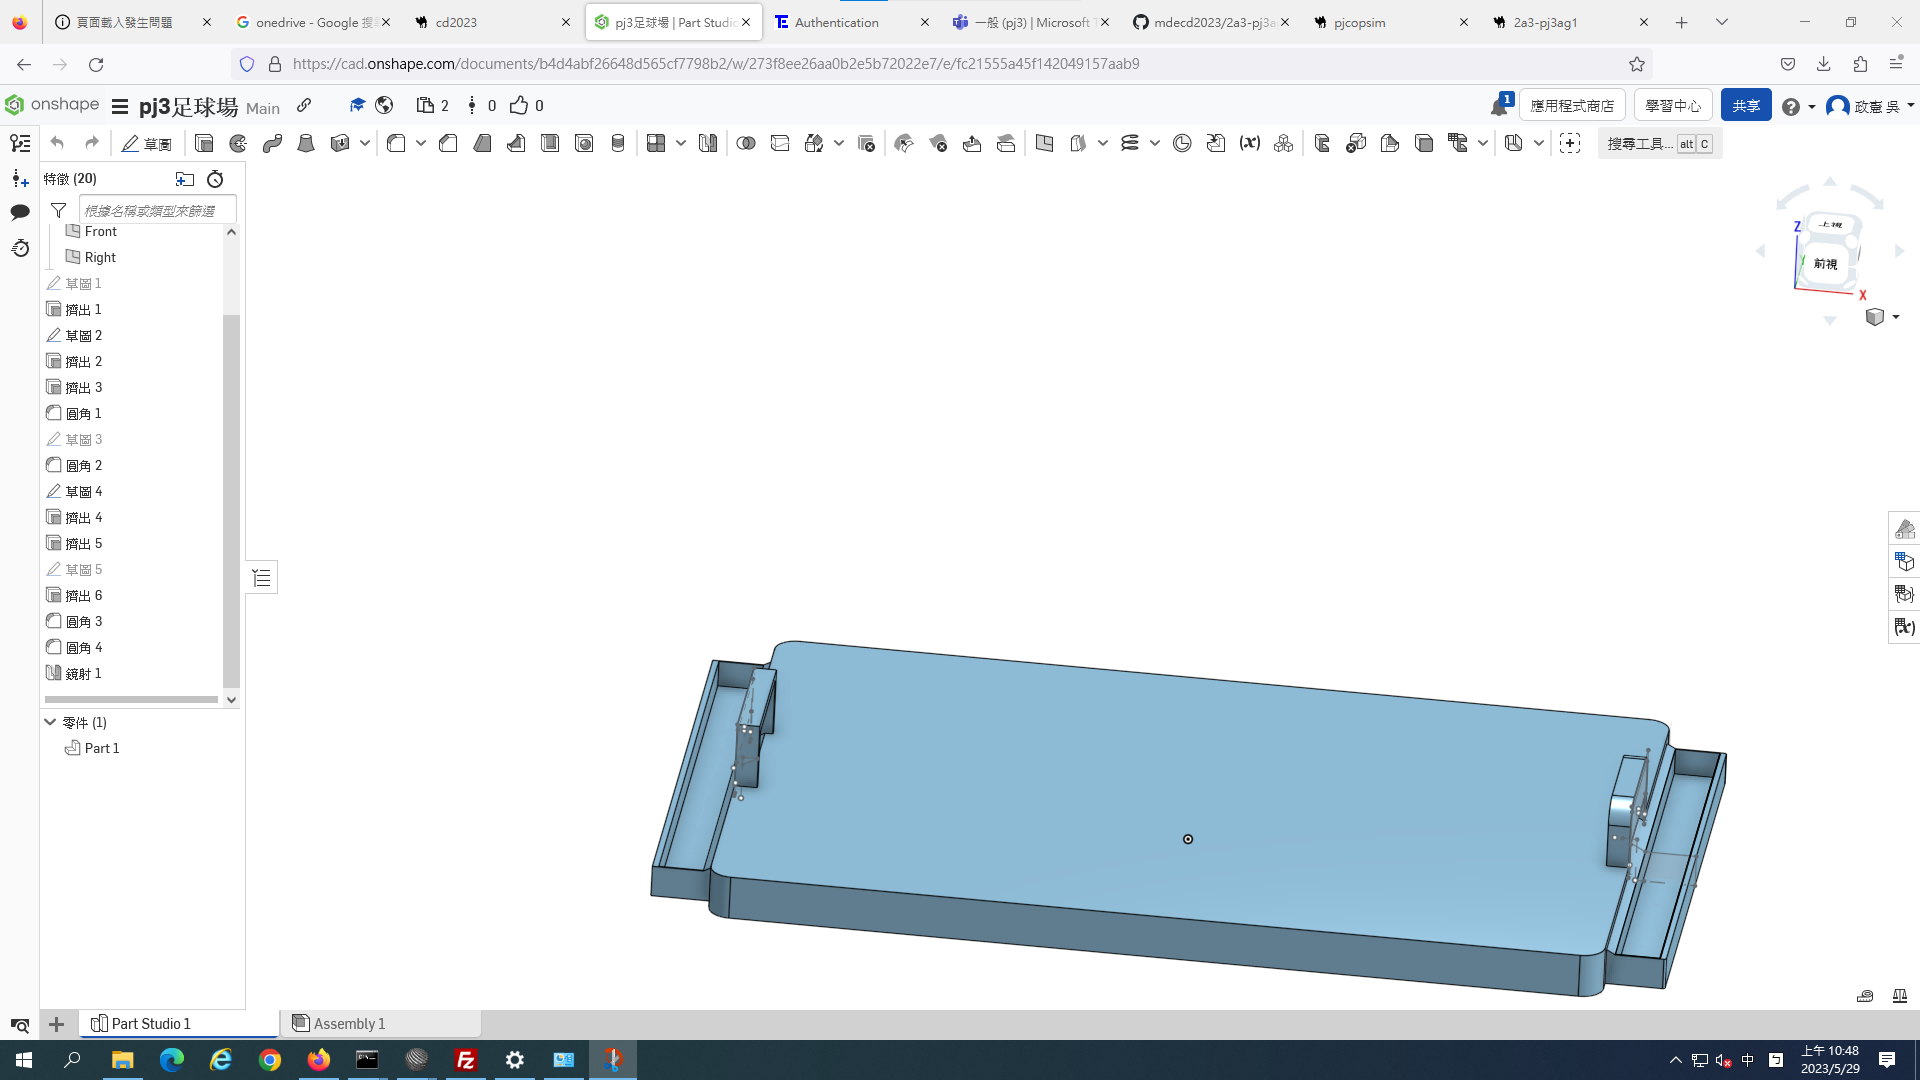
\includegraphics[width=8cm]{33333}
\caption{\Large 球場繪製}\label{球場繪製}
\end{center}
\end{figure}
\begin{figure}[hbt!]
\begin{center}
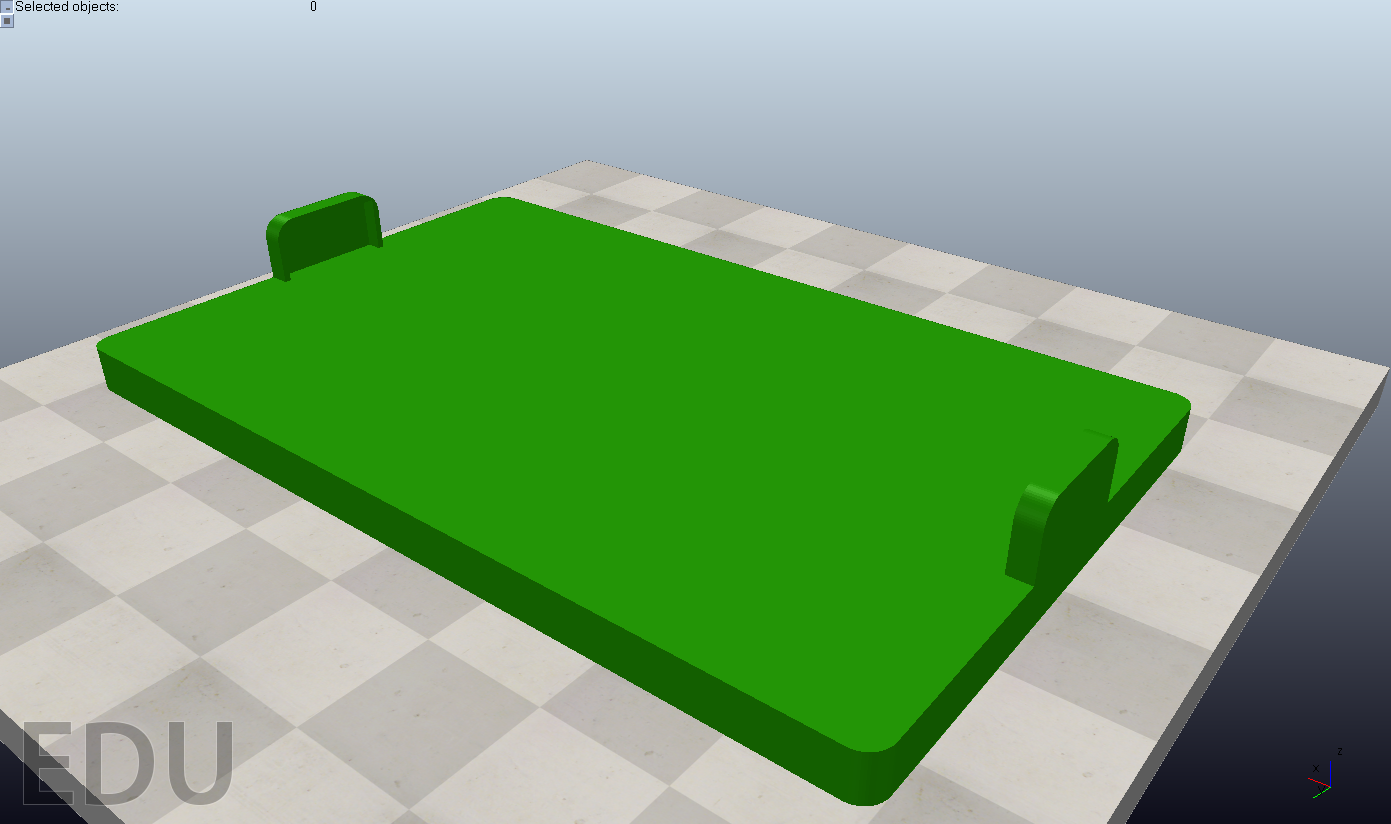
\includegraphics[width=8cm]{board}
\caption{\Large 導入球場}\label{導入球場}
\end{center}
\end{figure}
\newpage

\renewcommand{\baselinestretch}{0.5} %設定行距
\chapter{程式碼說明}
\renewcommand{\baselinestretch}{10.0} %設定行距
\pagenumbering{arabic} %設定頁號阿拉伯數字
\setcounter{page}{6}  %設定頁數
\fontsize{14pt}{2.5pt}\sectionef

\section{控制機器人程式}
此控制機器人程式利用 Python 語言。\\
\begin{figure}[hbt!]
\begin{center}
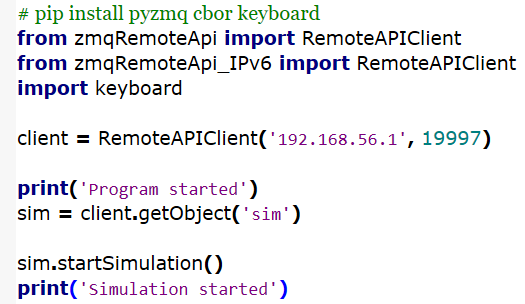
\includegraphics[height=6cm]{bubbleRob code 1}
\caption{\Large 控制機器人程式之一}\label{控制機器人程式之一}
\end{center}
\end{figure} 
使用 pip install pyzmq cbor keyboard 安裝了所需的套件,其中:\\
\begin{itemize}
\item \textbf{pyzmq} 用於建立 ZeroMQ 連線。
\item \textbf{cbor} 用於將資料序列化和反序列化。
\item \textbf{keyboard} 用於操控鍵盤事件。
\end{itemize}
使用 zmqRemoteApi 中的 IPv6  導入了用於建立與 CoppeliaSim 之間通訊的 Remote API 相關程式庫,使得可以通過程式碼控制仿真場景和物件,建立了一個 RemoteAPIClient 物件 client,並將 IP 和埠號分別作為 CoppeliaSim 的 IP 地址和連接埠。\\
這樣就建立了與 CoppeliaSim 的連線,使用 \texttt{client.getObject('sim')} 獲取了 CoppeliaSim 中的 sim 物件,該物件代表了整個仿真環境。透過這個物件,可以執行相關的仿真操作,再來透過  sim.startSimulation() 開始模擬。\\
\newpage

\begin{figure}[hbt!]
\begin{center}
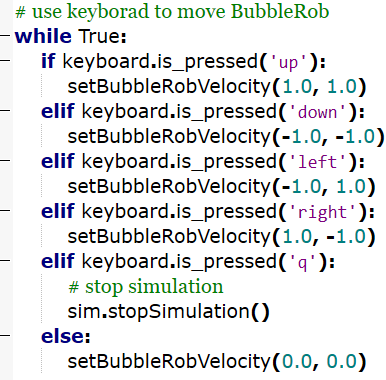
\includegraphics[height=8cm]{bubbleRob code 2}
\caption{\Large 控制機器人程式之二}\label{控制機器人程式之二}
\end{center}
\end{figure} 
這段程式碼是一個無窮迴圈,用於持續感測鍵盤並根據按鍵的狀態來控制機器人的運動。\\
如果按下 'up' 鍵,則呼叫 setBubbleRobVelocity(1.0, 1.0),將機器人的速度設定為正向。\\
如果按下 'down' 鍵,則呼叫 setBubbleRobVelocity(-1.0, -1.0),將機器人的速度設定為反向。\\
如果按下 'left' 鍵,則呼叫 setBubbleRobVelocity(-1.0, 1.0),將機器人的速度設定為左轉。\\
如果按下 'right' 鍵,則呼叫 setBubbleRobVelocity(1.0, -1.0),將機器人的速度設定為右轉。\\
如果按下 'q' 鍵,則停止仿真。若沒有按下上述任何按鍵,則呼叫 setBubbleRobVelocity(0.0, 0.0),將機器人的速度設定為零,即停止移動。\\
\newpage

\section{記分板程式}
此程式是使用 Lua 語言。\\
\begin{figure}[hbt!]
\begin{center}
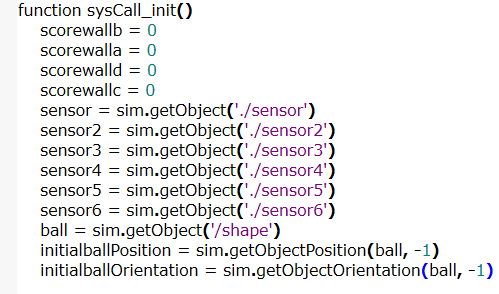
\includegraphics[height=6cm]{scorewall1}
\caption{\Large LED 記分板程式之一}\label{LED 記分板程式之一}
\end{center}
\end{figure} 
設定名稱為 sysCall init 的函數,在程式初始化時被呼叫。該函數的主要目的是初始化一些變數並取得物件的句柄。\\
1. scorewallb = 0、scorewalla = 0、scorewalld = 0、scorewallc = 0 用於初始化四個得分牆的變數,將初始值設為 0。\\
2. \texttt{sim.getObject} 獲取了各感測器及球的句柄。\\
3. \texttt{initialballPosition = sim.getObjectPosition(ball, -1)}:用於取得球體的初始位置。\\
4. \texttt{initialballOrientation = sim.getObjectOrientation(ball, -1)}:用於取得球體的初始方向。\\
\newpage

\begin{figure}[hbt!]
\begin{center}
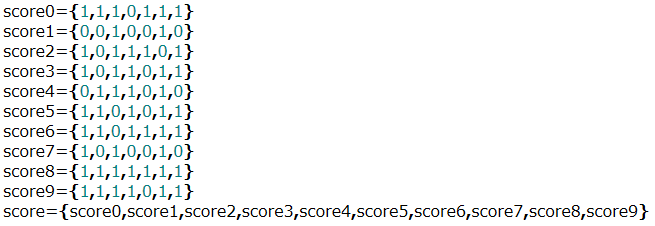
\includegraphics[height=5cm]{scorewall2}
\caption{\Large LED 記分板程式之二}\label{LED 記分板程式之二}
\end{center}
\end{figure} 
定義了一個包含十個元素的表格,每個元素都是由七個二進制數字(0或1)組成的列表。每個列表代表一個數字(0到9)的數字模式,而最後一行程式碼將這些數字模式放入一個名為 score 的表格中,以便在程式中進行使用。\\
\newpage

\begin{figure}[hbt!]
\begin{center}
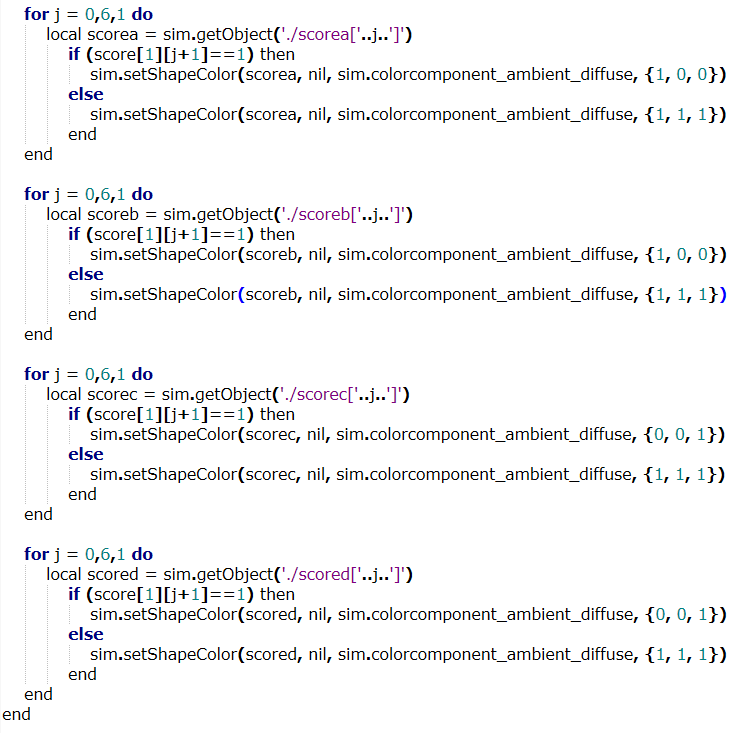
\includegraphics[height=10cm]{scorewall3}
\caption{\Large LED 記分板程式之三}\label{LED 記分板程式之三}
\end{center}
\end{figure}
這段程式碼是一個迴圈,用於對記分板進行顏色設定,根據事先定義的數字模式進行,迴圈的運行範圍是從0到6每次遞增1,在迴圈的每次迭代中,會執行以下操作:\\
1. scorewallb = 0、scorewalla = 0、scorewalld = 0、scorewallc = 0 用於初始化四個得分牆的變數,將初始值設為 0。\\
2. 創建一個指向記分板的參考是由迴圈變量 j 指定。\\
3. 檢查表格中的特定位置如果該位置的值等於 1,則使用 \texttt{sim.setShapeColor}函數設定記分板數字的顏色為紅色。\\
4. 如果該位置的值不等於 1,使用 \texttt{sim.setShapeColor}函數設定記分板數字的顏色為白色。\\
\newpage

\begin{figure}[hbt!]
\begin{center}
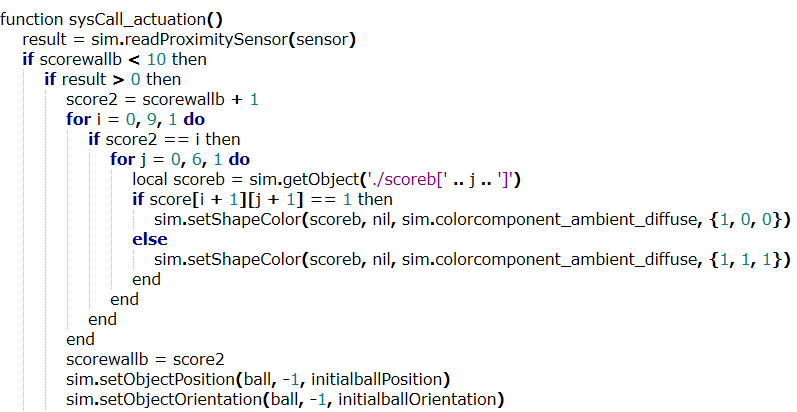
\includegraphics[height=8cm]{scorewall4}
\caption{\Large LED 記分板程式之四}\label{LED 記分板程式之四}
\end{center}
\end{figure} 
在此函式中,首先使用 \texttt{sim.readProximitySensor}函式讀取 sensor 的近接傳感器數值,並將結果存儲在 result 變數中,如果 scorewallb 小於 10,且如果 result 大於 0,表示與某個物體接觸。則執行以下操作:\\
1. 將 score2 設定為 scorewallb 加 1。\\
2. 進行一個迴圈從 0 到 9,每次遞增 1。\\
3. 如果 score2 等於 i 進行另一個迴圈從 0 到 6 每次遞增 1,創建一個指向 scoreb 的參考由迴圈 j 變量檢查 score 表格中的特定位置,如果該位置的值等於 1 使用 \texttt{sim.setShapeColor}函式設定 scoreb 物體的顏色為紅色,如果該位置的值不等於 1 使用 \texttt{sim.setShapeColor}函式設定 scoreb 物體的顏色為白色。\\
4. 更新 scorewallb 的值為 score2。\\
5. 使用 \texttt{sim.setObjectPosition} 函式將 ball 物體的位置設定為初始位置。\\
6. 使用 \texttt{sim.setObjectOrientation} 函式將 ball 物體的方向設定為初始方向。\\
\newpage

\begin{figure}[hbt!]
\begin{center}
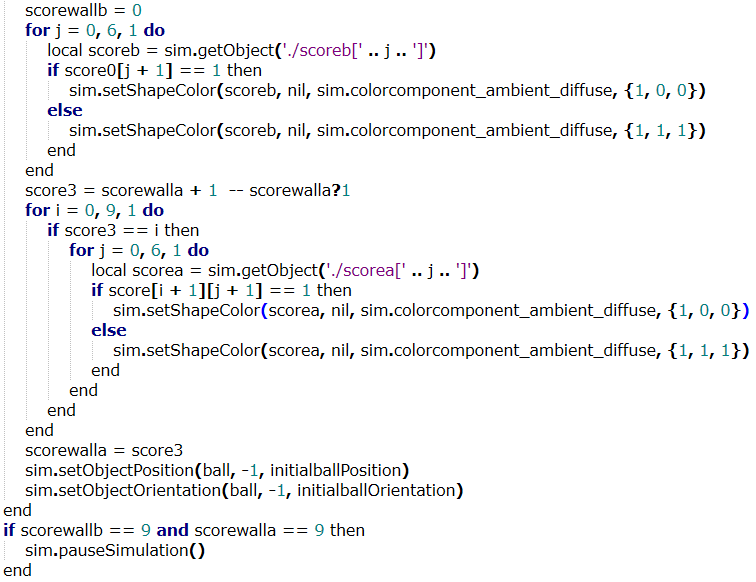
\includegraphics[height=10cm]{scorewall5}
\caption{\Large LED 記分板程式之五}\label{LED 記分板程式之五}
\end{center}
\end{figure} 
反之如果 scorewallb 大於 9 則執行以下操作:\\
1. 將 scorewallb 的值設定為 0。\\
2. 進行一個迴圈從 0 到 6,每次遞增 1 創建一個指向 scoreb 物體的參考,該物體是由迴圈變量 j 指定的物體,如果該位置的值等於 1 使用 \texttt{sim.setShapeColor}函式設定 scoreb 物體的顏色為紅色,如果該位置的值不等於 1 使用 \texttt{sim.setShapeColor}函式設定 scoreb 物體的顏色為白色。\\
3. 將 score3 設定為 scorewalla 加 1。\\
4. 更新 scorewallb 的值為 score2。\\
5. 進行一個迴圈從 0 到 9,每次遞增 1 ,如果 score3 等於 i 進行一個迴圈從 0 到 6,每次遞增 1 創建一個指向 scoreb 物體的參考,該物體是由迴圈變量 j 指定的物體,如果該位置的值等於 1 使用 \texttt{sim.setShapeColor}函式設定 scoreb 物體的顏色為紅色,如果該位置的值不等於 1 使用 \texttt{sim.setShapeColor}函式設定 scoreb 物體的顏色為白色。\\
6. 更新 scorewalla 的值為 score3。\\
7. 使用 \texttt{sim.setObjectPosition} 函式將 ball 物體的位置設定為初始位置。\\
8. 使用 \texttt{sim.setObjectOrientation} 函式將 ball 物體的方向設定為初始方向。\\
9. 程式碼檢查兩個變數 scorewallb 和 scorewalla 是否都等於 9。如果兩個變數的值都等於 9 用  \texttt{sim.pauseSimulation()} 函式暫停仿真。\\
而另一隊記分板也是使用一樣的程式只是更改名稱。\\

\begin{figure}[hbt!]
\begin{center}
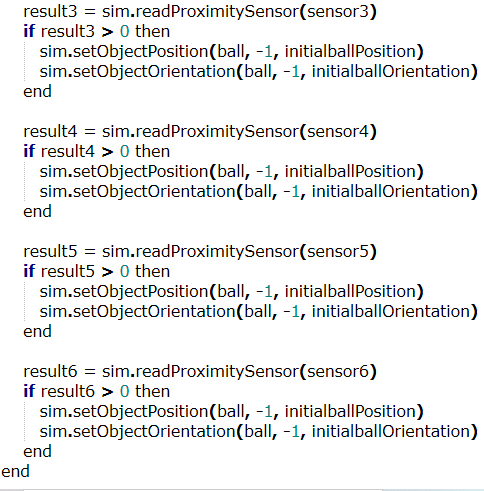
\includegraphics[height=8cm]{scorewall6}
\caption{\Large LED 記分板程式之六}\label{LED 記分板程式之六}
\end{center}
\end{figure} 
如果感測器感測到物體則執行以下操作:\\
1. 使用 \texttt{sim.setObjectPosition} 函式將 ball 物體的位置設定為初始位置。\\
2. 使用 \texttt{sim.setObjectOrientation} 函式將 ball 物體的方向設定為初始方向。\\
\newpage

\begin{figure}[hbt!]
\begin{center}
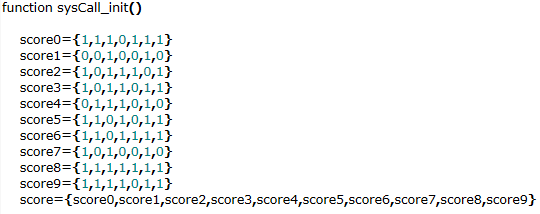
\includegraphics[height=8cm]{time1}
\caption{\Large 計時器程式之一}\label{計時器程式之一}
\end{center}
\end{figure} 
沿用了記分板的程式:\\
設定名稱為 sysCall init 的函數,在程式初始化時被呼叫。該函數的主要目的是初始化一些變數並取得物件的句柄。\\定義了一個包含十個元素的表格,每個元素都是由七個二進制數字(0或1)組成的列表。每個列表代表一個數字(0到9)的數字模式,而最後一行程式碼將這些數字模式放入一個名為 score 的表格中,以便在程式中進行使用。\\
\newpage

\begin{figure}[hbt!]
\begin{center}
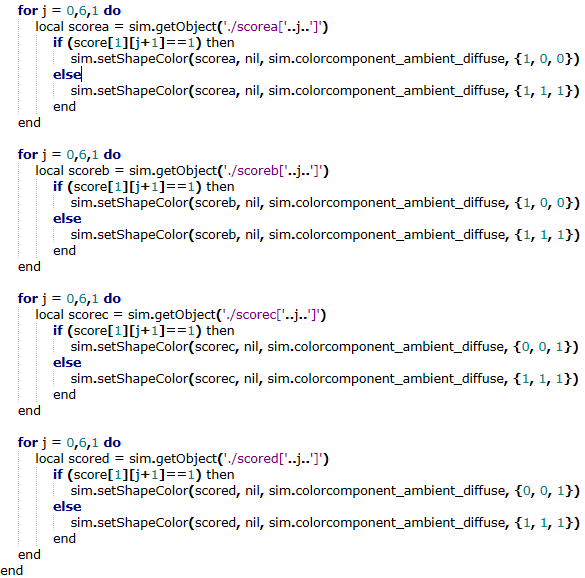
\includegraphics[height=8cm]{time2}
\caption{\Large 計時器程式之二}\label{計時器程式之二}
\end{center}
\end{figure} 
沿用了記分板的程式:\\
這段程式碼是一個迴圈,用於對記分板進行顏色設定,根據事先定義的數字模式進行,迴圈的運行範圍是從0到6每次遞增1,在迴圈的每次迭代中,會執行以下操作:\\
1. scorewallb = 0、scorewalla = 0、scorewalld = 0、scorewallc = 0 用於初始化四個得分牆的變數,將初始值設為 0。\\
2. 創建一個指向記分板的參考是由迴圈變量 j 指定。\\
3. 檢查表格中的特定位置如果該位置的值等於 1,則使用 \texttt{sim.setShapeColor}函數設定記分板數字的顏色為紅色。\\
4. 如果該位置的值不等於 1,使用 \texttt{sim.setShapeColor}函數設定記分板數字的顏色為白色。\\
\newpage

\begin{figure}[hbt!]
\begin{center}
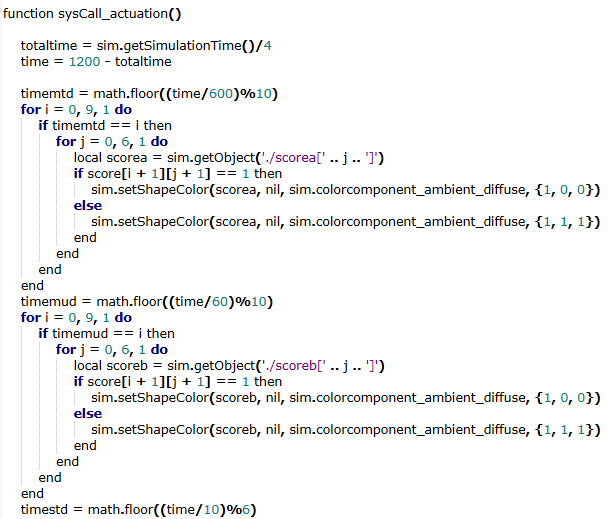
\includegraphics[height=8cm]{time3}
\caption{\Large 計時器程式之三}\label{計時器程式之三}
\end{center}
\end{figure} 
1. totaltime = \texttt{sim.getSimulationTime()/4}: 計算從模擬開始到現在的總時間,並除以 4(為了調整時間的比例)。\\
2. \texttt{time = 1200 - totaltime}:根據總時間計算剩餘時間,1200 這部分可依照自己需求去修改。\\
3. \texttt{timemtd = math.floor((time/600)\%10):根據剩餘時間計算十位數分鐘數字,math.floor 函數用於將計算結果向下取整,\% 表示取模運算符號,這裡是將時間除以 600 取其餘數,再取該餘數的整數部分。\\
4. \texttt{for i = 0, 9, 1 do}:進行一個迴圈從 0 到 9,每次遞增 1。\\
5. \texttt{if timemtd == i then}:檢查十位數分鐘是否等於當前迴圈數字。\\
6. 在內部循環 \texttt{for j = 0, 6, 1 do} 中,進行顯示相關的操作。\\
7. \texttt{local scorea = sim.getObject('./scorea[' .. j .. ']')}:獲取記分板十位數分鐘的句柄。\\
8. \texttt{if score[i + 1][j + 1] == 1 then}:檢查特定位置上的數字是否為 1(即該位置需要亮起)。\\
9. \texttt{sim.setShapeColor(scorea, nil, sim.colorcomponent_ambient_diffuse, {1, 0, 0})}:設置該顯示元素的顏色為紅色(表示亮起)。\\
10. \texttt{sim.setShapeColor(scorea, nil, sim.colorcomponent_ambient_diffuse, {1, 1, 1})}:設置該顯示元素的顏色為白色(表示熄滅)。\\
11. \texttt{timemtd = math.floor ((time/60)\%600)}:分別用於計算十位數分鐘數字,並根據結果進行相應的顯示操作。\\
個位數分鐘與上面程式相同唯一不同的是 \texttt{timemud = math.floor((time/10)\%60)}用於計算個位數分鐘數字,並根據結果進行相應的顯示操作。\\
\newpage

\begin{figure}[hbt!]
\begin{center}
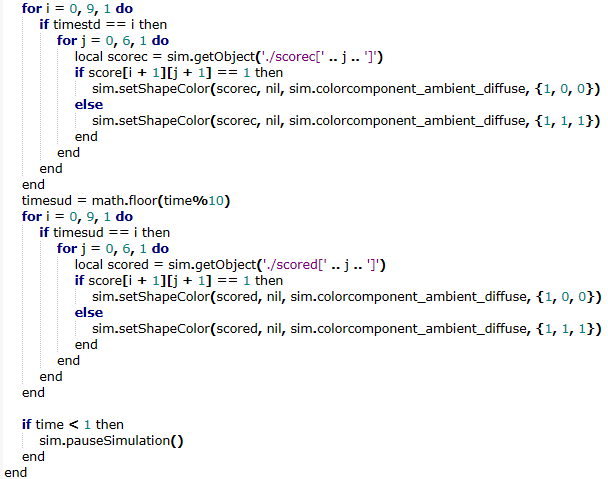
\includegraphics[height=8cm]{time4}
\caption{\Large 計時器程式之四}\label{計時器程式之四}
\end{center}
\end{figure} 
程式與十位、個位數分鐘相同唯一不同的是 
1. \texttt{timestd = math.floor((time/10)\%10)} 用於計算十位數秒鐘數字,並根據結果進行相應的顯示操作。\\
2. \texttt{timesud = math.floor(time/10)} 用於計算個位數秒鐘數字,並根據結果進行相應的顯示操作。\\
3. 當時間小於 1 時停止模擬。\\
\newpage
\renewcommand{\baselinestretch}{1.0} %設定行距
%\input{4_server.tex}
\chapter{場景模擬}
\renewcommand{\baselinestretch}{10.0} %設定行距
\pagenumbering{arabic} %設定頁號阿拉伯數字
\setcounter{page}{7}  %設定頁數
\fontsize{14pt}{2.5pt}\sectionef
\section{摘要}
  完成球員及程式碼設定後,接著建立模擬場景,添加場地、球員、計時器、 LED 記分板和機械式轉盤記分板\\
\section{統整場景}
  在球場周圍設置感測器球碰到會返回中心,放入 8 名球員,以兩色分為兩隊。\\
\begin{figure}[hbt!]
\begin{center}
\includegraphics[height=8cm]{60}
\caption{\Large 球場建立}\label{總2}
\end{center}
\end{figure}

  和計時器、LED計分板和機械式記分板。\\
\begin{figure}[hbt!]
\begin{center}
\includegraphics[height=15cm]{61}
\caption{\Large 球場全貌}\label{總}
\end{center}
\end{figure}
\renewcommand{\baselinestretch}{1} %設定行距
\chapter{組員連線}
\renewcommand{\baselinestretch}{10.0} %設定行距
\pagenumbering{arabic} %設定頁號阿拉伯數字
\setcounter{page}{21}  %設定頁數
\fontsize{14pt}{2.5pt}\sectionef
\section{摘要}
  完成場景建設後,要實施跨電腦連線對戰,使用zmqRemoteAPI 寫的程式和下載 CoppeliaSim(4.5.1) 支援 IPv6 版本,zmq 中也需具備 IPv6 環境,然後由組長開起場景,組員跨網路控制各自的編號球員開始對戰。\\
\section{連線說明-防火牆}
  從控制台將防火牆都關閉,點開進階設定,組長設定"輸入規則"、組員設定"輸出規則"。新增規則 / 連接埠 / TCP(傳輸控制協定Port) / 特定連接埠 23000-23050,選擇允許連線。\\
\begin{figure}[hbt!]
\begin{center}
\includegraphics[height=10cm]{防3}
\caption{\Large 控制台連接埠}\label{防3}
\end{center}
\end{figure}
\section{連線說明-IPv6}
  設定網路 IPv6 位址。\\
\begin{figure}[hbt!]
\begin{center}
\includegraphics[height=10cm]{防9}
\caption{\Large 網路 IPv6 位置}\label{防9}
\end{center}
\end{figure}

  接著在 zmq 的 localhost 處打上組長的 IPv6 位置連線。\\
\newpage
\begin{figure}[hbt!]
\begin{center}
\includegraphics[height=10cm]{連1}
\caption{\Large 組長 IPv6 }\label{連1}
\end{center}
\end{figure}
  最後在瀏覽器輸入 http://[組長 IP 位置]:23020,即可看到組長的場景。
%\input{7_discussions.tex}
%=---------------------參考文獻----------------------=%
%=---------------附錄-----------------=%
\newpage
\end{document}
